\section{Mapping Between SBOL 1, SBOL 2, and SBOL3}
\label{sec:mapping}

In broad strokes, the SBOL 1 standard focused on conveying physical, structural information, whereas SBOL 2 expanded the scope to include functional aspects as well.  
The physical information about a designed genetic construct includes the order of its constituents and their descriptions. 
Specifying the exact locations of these constituents and their sequences allows genetic constructs to be defined unambiguously and reused in other designs. 
SBOL 2 extended SBOL 1 in several ways: it extends physical descriptions to include entities beyond DNA sequences, and it added support for functional descriptions of designs.  
SBOL 3 refines the data model to simplify the representation of common use cases.

\subsection{Mapping between SBOL 1 and SBOL 2}

\ref{SBOL1TO2} depicts the mapping of SBOL 1.1 classes to SBOL 2.x classes, indicating corresponding classes/properties by color.
The SBOL 2.x \external{Model} and \external{ModuleDefinition} classes have no SBOL 1.1 equivalent, and thus are not shown.
The mapping from SBOL 1.1 to SBOL 2.x proceeds as follows:
\begin{itemize}
\item SBOL 1.1 \external{Collection} objects containing \external{DnaComponent} objects map to SBOL 2.x \external{Collection} objects that contain \external{CompenentDefinition} objects with DNA \sbolmult{types:CD}{types} properties.
\item SBOL 1.1 \external{DnaComponent} objects map to SBOL 2.x \external{CompenentDefinition} objects with DNA \sbolmult{types:CD}{types} properties.
\item SBOL 1.1 \external{DnaSequence} objects map to an SBOL 2.x \external{Sequence} objects with \external{IUPAC DNA} \external{encoding} properties.
\item SBOL 1.1 \external{SequenceAnnotation} objects with \external{bioStart} and \external{bioEnd} properties map to SBOL 2.x\\
\external{SequenceAnnotation} objects that contain \external{Range} objects.
\item SBOL 1.1 \external{SequenceAnnotation} objects that lack \external{bioStart} and \external{bioEnd} properties map to an SBOL 2.x \external{SequenceFeature} objects that contain \external{GenericLocation} objects.
\item Each SBOL 1.1 \external{SequenceAnnotation} also maps to an SBOL 2.x \external{Component}, which represents the instantiation or usage of the appropriate \external{CompenentDefinition}.
\item Each SBOL 1.1 \external{precedes} property maps to an SBOL 2.x \external{SequenceConstraint} that specifies a precedes \external{restriction} property.
\end{itemize}

\begin{figure*}[h]
\begin{center}
  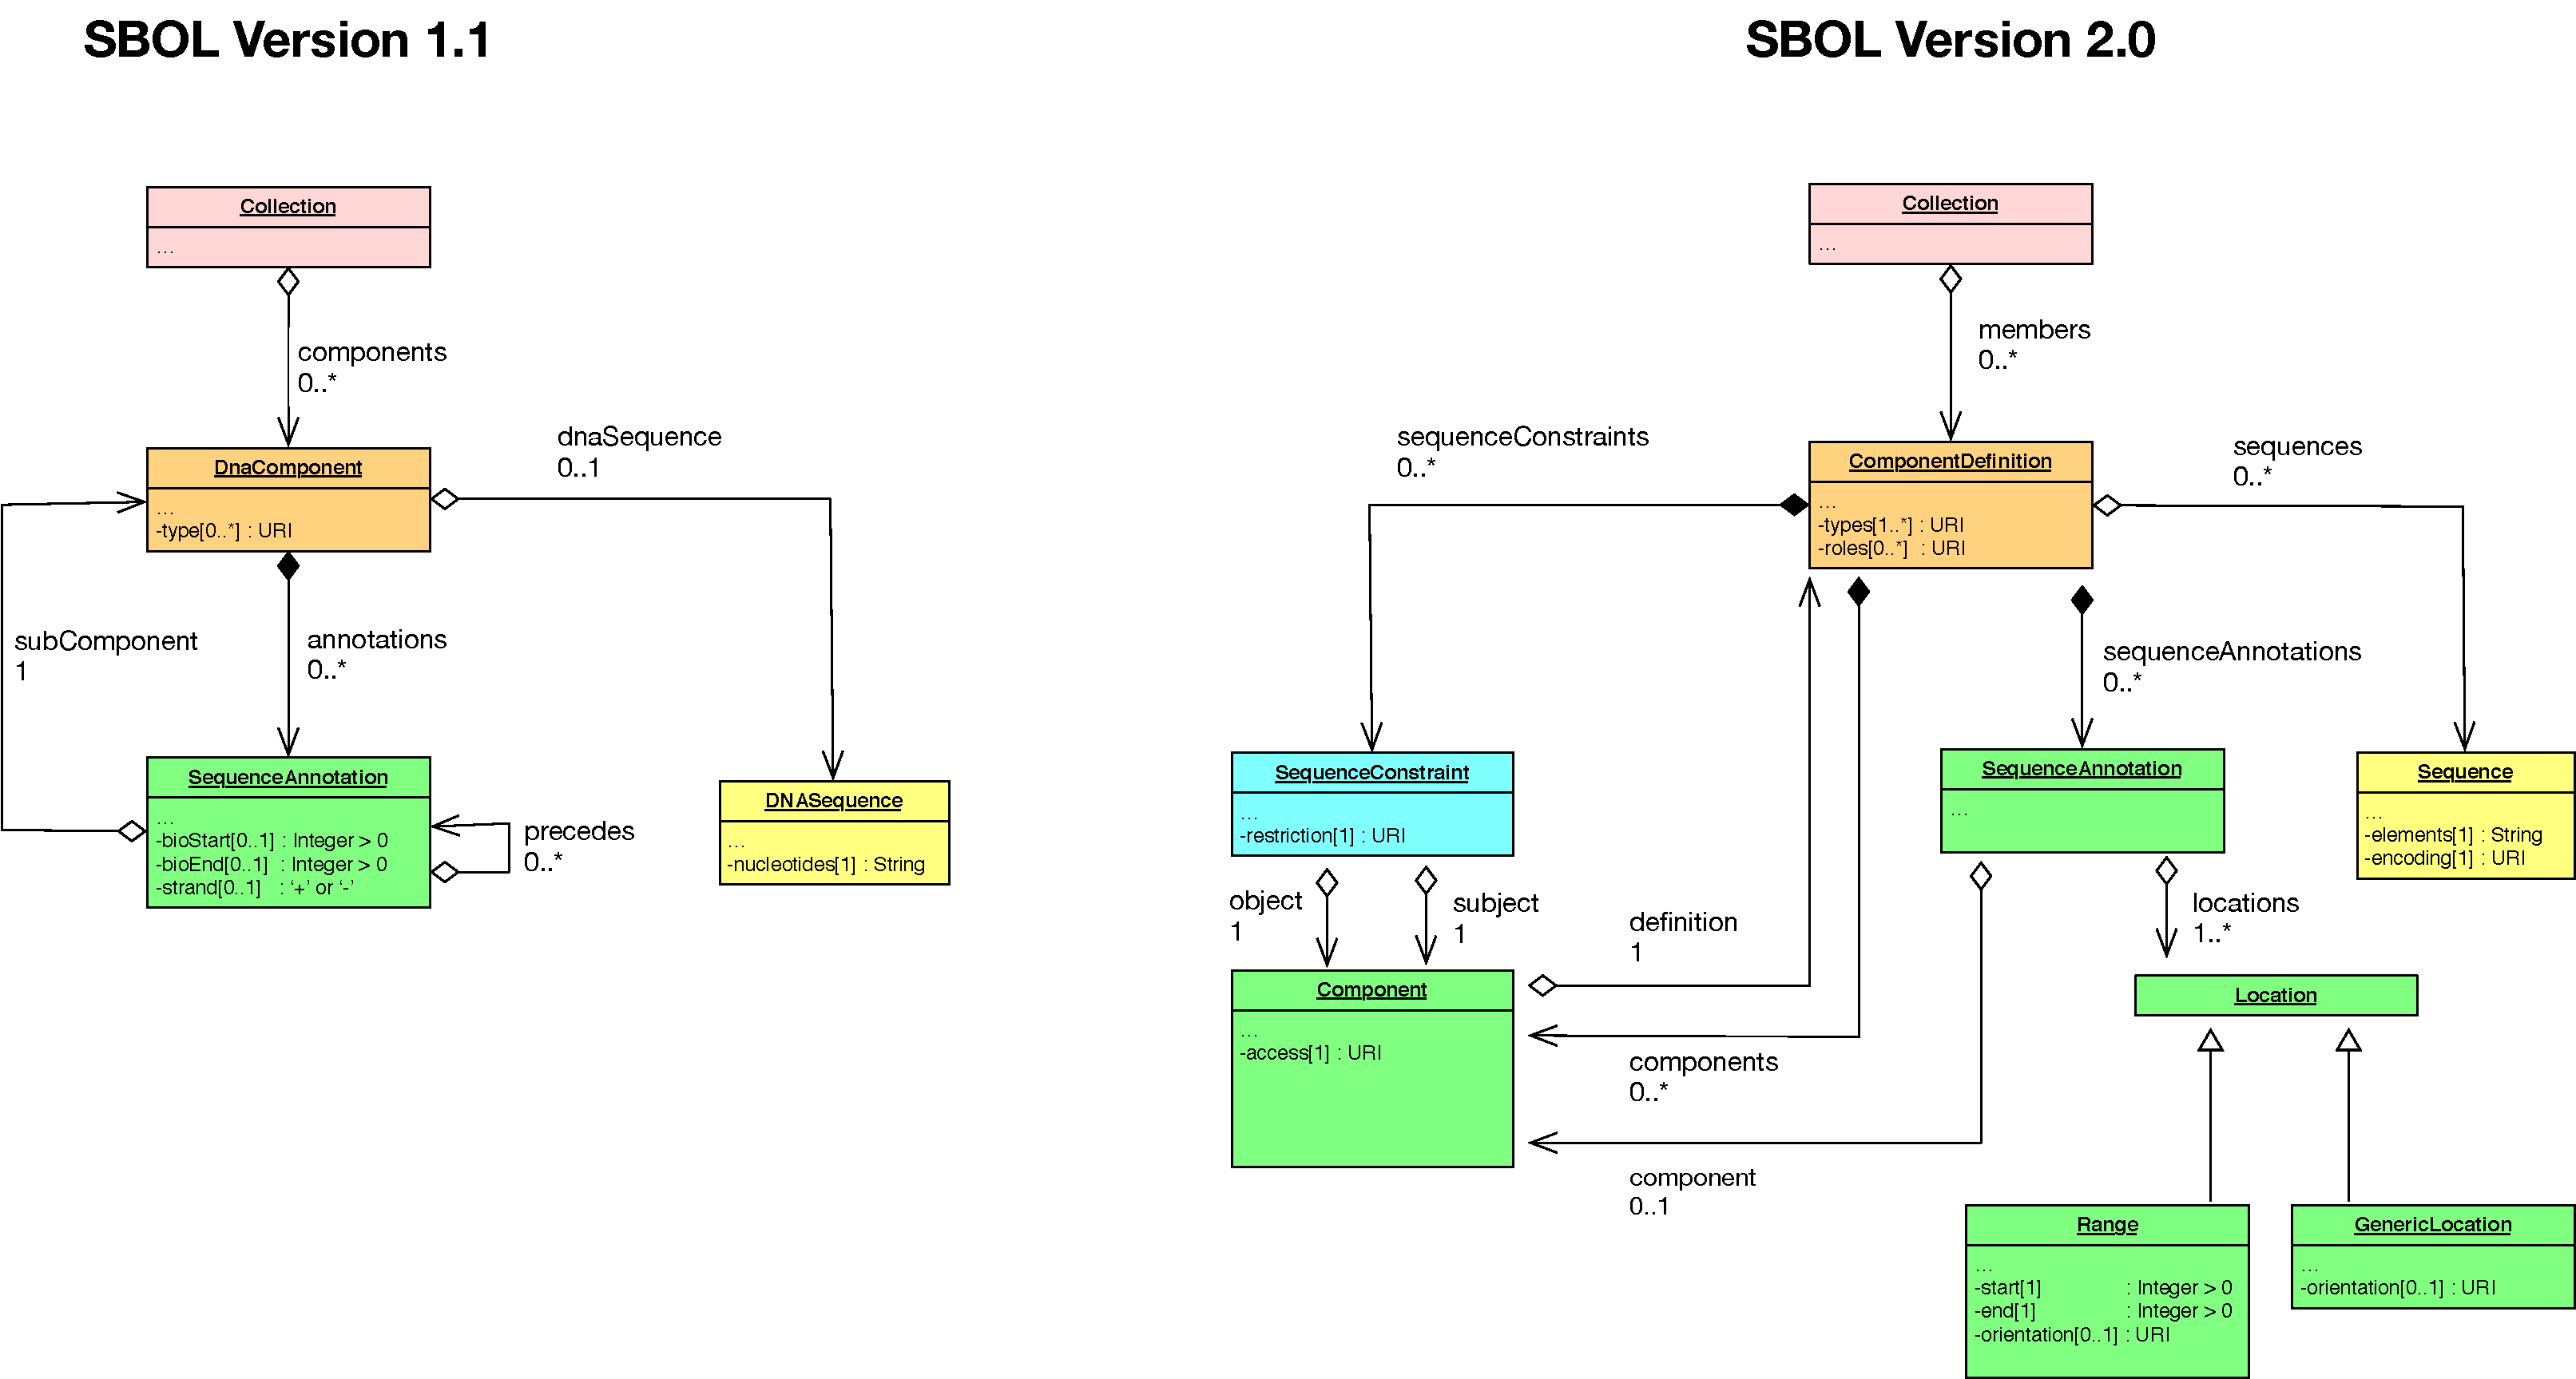
\includegraphics[width=\textwidth]{images/sbol_v1_to_v2}
\end{center}
\caption{\label{SBOL1TO2}The mapping from the SBOL 1.1 data model to the SBOL 2.x  data model, indicating corresponding classes/properties by color.}
\end{figure*}



\subsection{Mapping between SBOL 2 and SBOL 3}

\ref{SBOL2TO3} depicts the mapping of SBOL 2.3 classes to SBOL 3.x classes, indicating corresponding classes/properties by color.   
The SBOL 3.x \sbol{Namespace} class has no SBOL 2.x equivalent, and thus is not shown.
The SBOL 2.x \sbol{Attachment}, \sbol{CombinatorialDerivation}, \sbol{ExperimentalData}, \sbol{Experiment}, \sbol{Implementation}, \sbol{Model}, \sbol{Participation}, and \\ \sbol{VariableComponent} classes are omitted or abstracted, since they are essentially unchanged in SBOL 3.x except for the following property renamings:
\begin{itemize}
\item In \sbol{VariableComponent}, the SBOL 2.x \external{operator} property maps to the SBOL 3.x \sbol{cardinality} property.
\item In \sbol{Experiment}, the SBOL 2.x \external{experimentalData} property maps to the SBOL 3.x \sbol{member} property.
\end{itemize}

The mapping from SBOL 2.x to SBOL 3.x proceeds as follows:
\begin{itemize}
    \item SBOL 2.x \external{ComponentDefinition} objects map to SBOL 3.x \sbol{Component} objects.  The \sbol{type} property is mapped according to  \ref{tbl:component_type_mapping}.
    \item SBOL 2.x \external{ModuleDefinition} objects map to SBOL 3.x \sbol{Component} objects with a \sbol{type} of \texttt{SBO:0000241} (functional entity)
    \item Every \external{FunctionalComponent} in an SBOL 2.x \external{ModuleDefinition} with a "direction" property that is not "none" is listed in the \sbol{Interface} of its SBOL 3.x \sbol{Component}. The mapping from direction to interface properties is: "in"-->"inputs", "out"-->"outputs", "inout" --> "nondirectional". Finally, every Component with "access"="public" and "direction"="none" is listed as "nondirectional" in the Interface.
    \item Every \external{Component} in an SBOL 2.x \external{ComponentDefinition} with "access"="public" is listed as "nondirectional" in the \sbol{Interface} of its SBOL 3.x \sbol{Component}.
    \item SBOL 2.x \external{Component}, \external{Module}, and \external{FunctionalComponent} objects map to SBOL 3.x \sbol{SubComponent} objects
    \item SBOL 2.x \external{SequenceAnnotation} objects map to SBOL 3.x \sbol{SequenceFeature} objects if they do not have a \external{component}. If they do have a \external{component}, their locations are added to the corresponding SBOL3 \sbol{SubComponent}.
%    \item \external{Location} objects are assigned an \sbol{order} integer.  In the case of multiple locations, the order may be inferred, e.g. from the \external{start} and \external{end} properties of ranges.  However, such behavior is tooling-specific.
    \item SBOL 2.x \external{SequenceConstraint} objects map to SBOL 3.x \sbol{Constraint} objects
    \item SBOL 2.x \external{MapsTo} objects are converted by transforming each \external{MapsTo} into two SBOL 3.x objects: \\ a \sbol{ComponentReference} and a \sbol{Constraint}.
      \begin{itemize}
      \item For the \sbol{ComponentReference}, the \sbol{inChildOf} attribute of this \sbol{ComponentReference} attribute references the object that has the \external{MapsTo} as a child, and the \sbol{hasFeature} attribute references the object referred to by the \external{remote} attribute from the \external{MapsTo} object.
      \item The \sbol{Constraint} links this \sbol{ComponentReference} and the \sbol{SubComponent} referred to be the \external{local} attribute from the \external{MapsTo} object.  The property values of the \sbol{Constraint} depend on the value of the \external{refinement} value for the \external{MapsTo} object:
      	\begin{itemize}
	\item If the refinement is \external{useRemote}, then the \sbol{restriction} is \external{replaces}, the \sbol{subject} is the \\ \sbol{ComponentReference} and the \sbol{object} is the \sbol{SubComponent}.
	\item If the refinement is \external{useLocal}, then the \sbol{restriction} is \external{replaces}, the \sbol{subject} is the \sbol{SubComponent} and the \sbol{object} is the \sbol{ComponentReference}.
	\item If the refinement is \external{verifyIdentical}, then the \sbol{restriction} is \external{verifyIdentical}, the \sbol{subject} is the \sbol{ComponentReference} and the \sbol{object} is the \sbol{SubComponent}.
	\item The \external{merge} \external{refinement} was never well defined and rarely if ever used, so it has been removed from SBOL 3.x.  If a \external{merge} is encountered, it SHOULD be handled as a \external{useRemote}.      
        \end{itemize}
     \item As an OPTIONAL optimization, if the \sbol{SubComponent} referred to be the \external{local} property of the \external{MapsTo} is a ``placeholder'' with no significant content apart from its \sbol{MapsTo} relationships, then it may be eliminated, all objects that pointed to it can point directly to the new \sbol{ComponentReference} instead, and all transitive constraints using it as a bridge reduced to link the endpoints directly. 
     \end{itemize}
\end{itemize}


\begin{table}[ht]
  {\scriptsize
  \begin{edtable}{tabular}{ll}
    \toprule
    \textbf{SBOL 2.x Type} & \textbf{SBOL 3.x Type} \\
    \midrule
      \url{http://www.biopax.org/release/biopax-level3.owl\#Dna} & \url{https://identifiers.org/SBO:0000251 (DNA)}\\
      \url{http://www.biopax.org/release/biopax-level3.owl\#DnaRegion} & \url{https://identifiers.org/SBO:0000251} (DNA)\\
      \url{http://www.biopax.org/release/biopax-level3.owl\#Rna} & \url{https://identifiers.org/SBO:0000250} (RNA)\\
      \url{http://www.biopax.org/release/biopax-level3.owl\#RnaRegion} & \url{https://identifiers.org/SBO:0000250} (RNA)\\
      \url{http://www.biopax.org/release/biopax-level3.owl\#Protein} & \url{https://identifiers.org/SBO:0000252} (Protein)\\
      \url{http://www.biopax.org/release/biopax-level3.owl\#SmallMolecule} & \url{https://identifiers.org/SBO:0000247} (Simple Chemical)\\
      \url{http://www.biopax.org/release/biopax-level3.owl\#Complex} & \url{https://identifiers.org/SBO:0000253} (Non-covalent Complex)\\
    \bottomrule
  \end{edtable}
  }
  \caption{Mapping of SBOL2 ComponentDefinition types to SBOL3 Component types}
 \label{tbl:component_type_mapping}
\end{table}


\begin{figure*}[h]
	\begin{subfigure}{\textwidth}
		\centering
		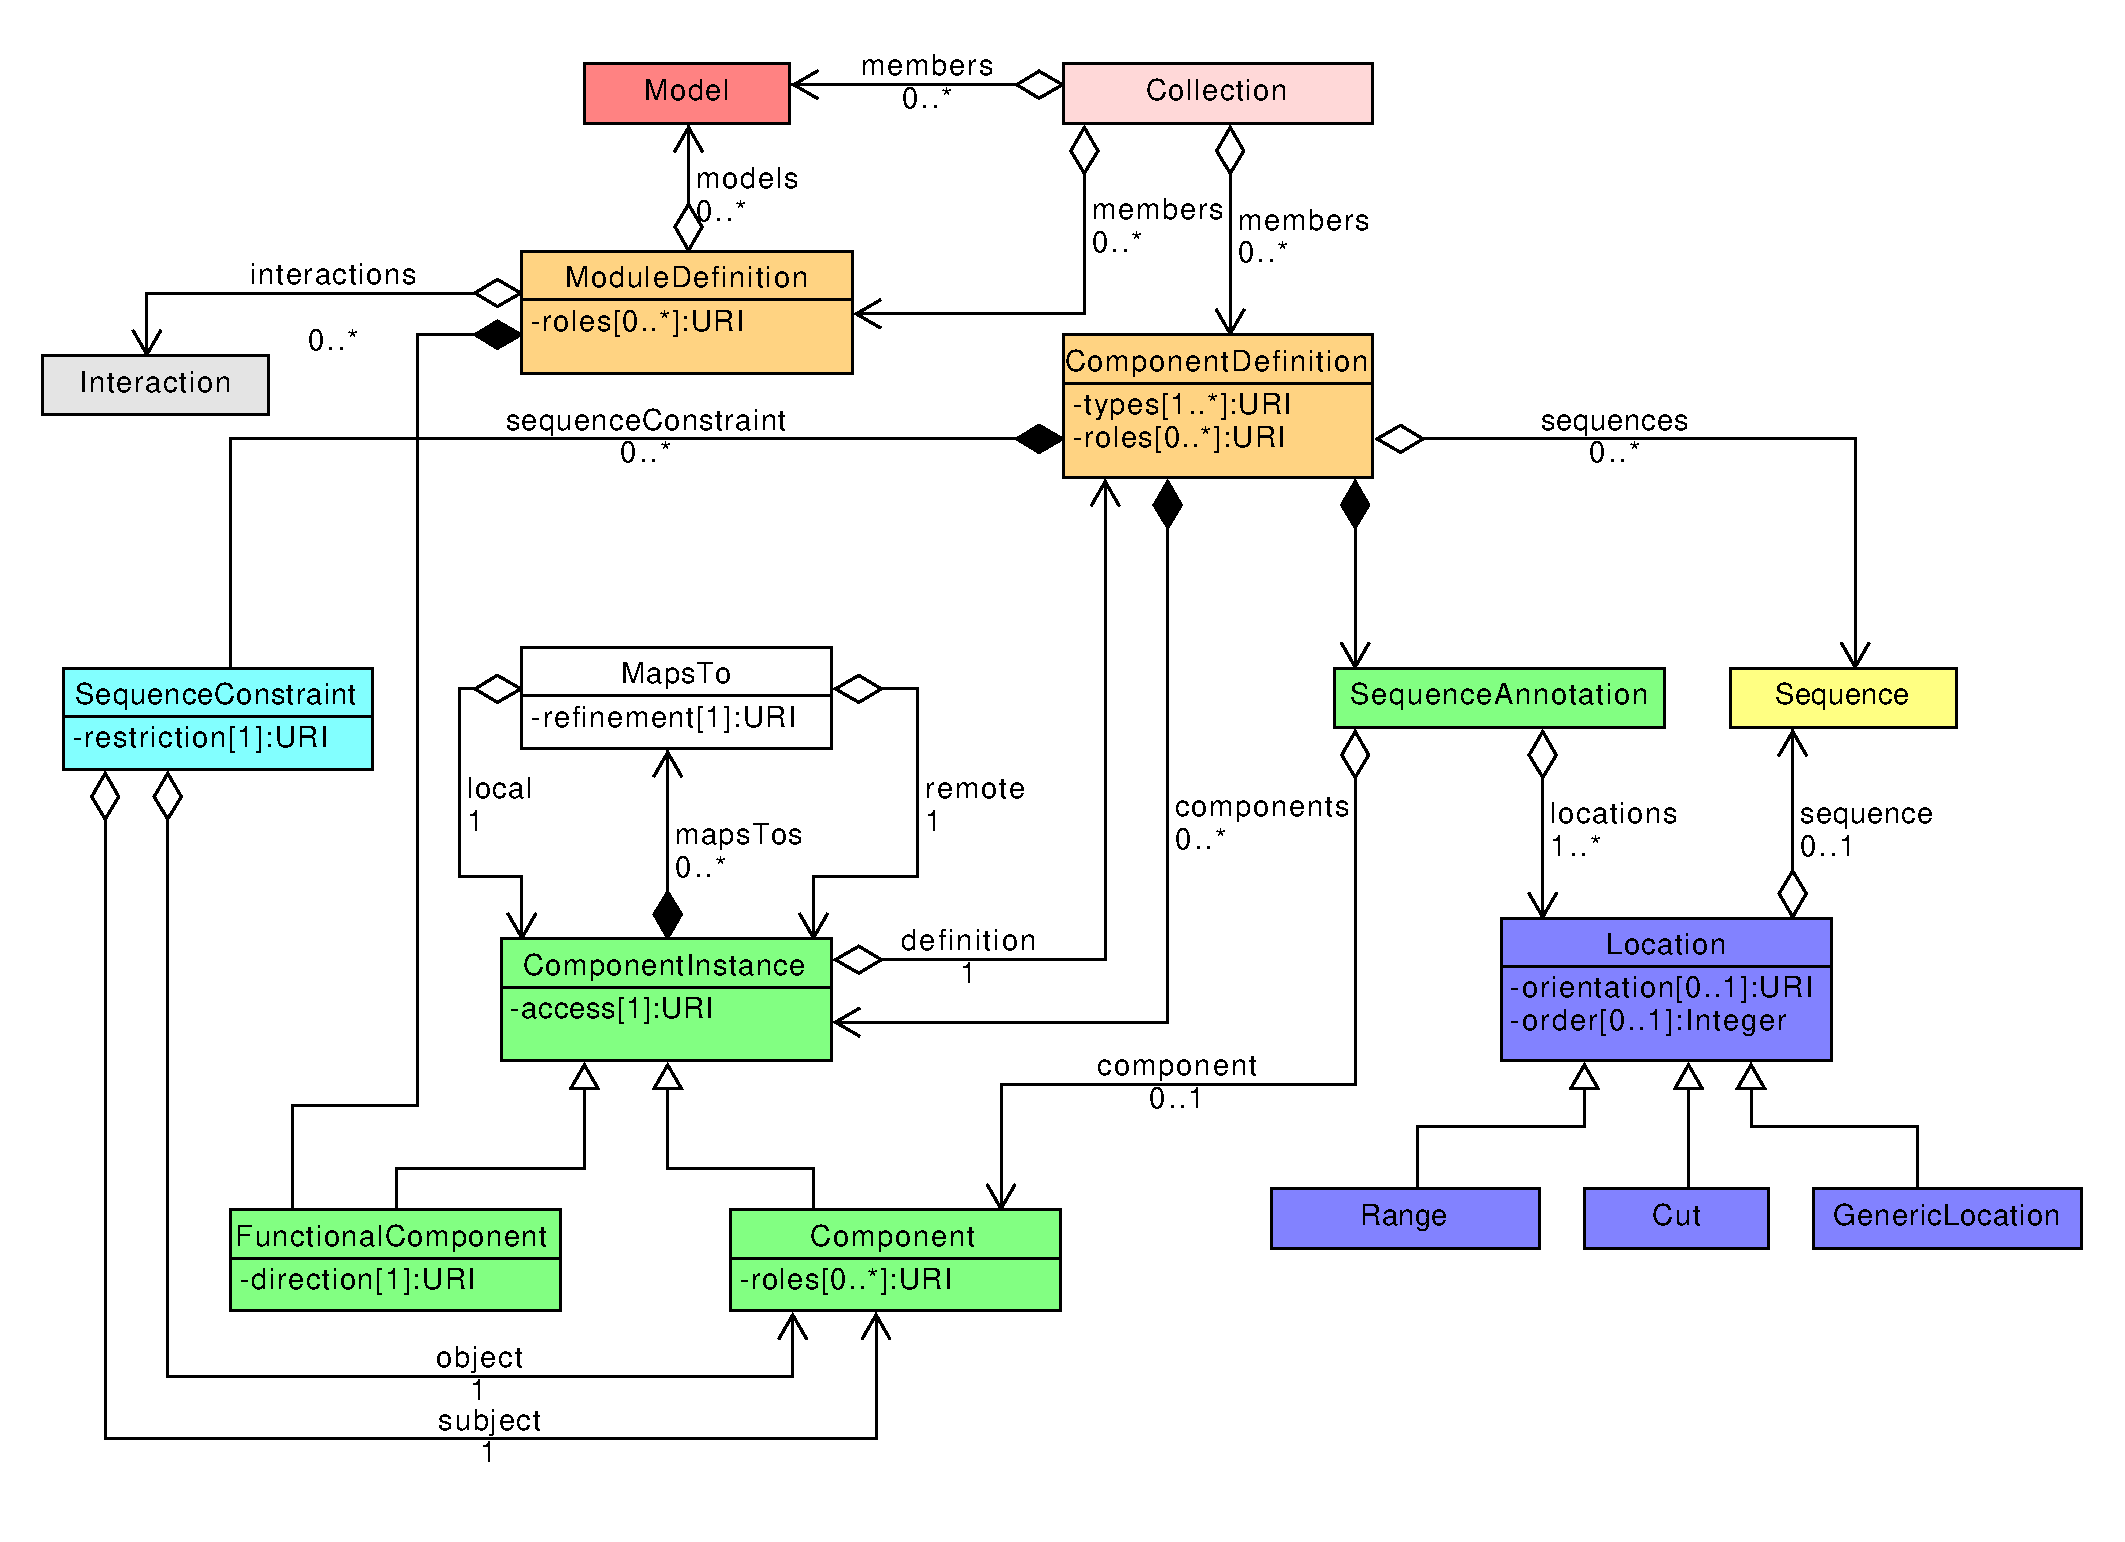
\includegraphics[width=0.8\linewidth]{uml/sbol_v2_to_v3_left_subfigure}  
		\caption{SBOL 2.3}
		\label{fig:sub-first}
              \end{subfigure}\\
              \begin{subfigure}{\textwidth}
		\centering
		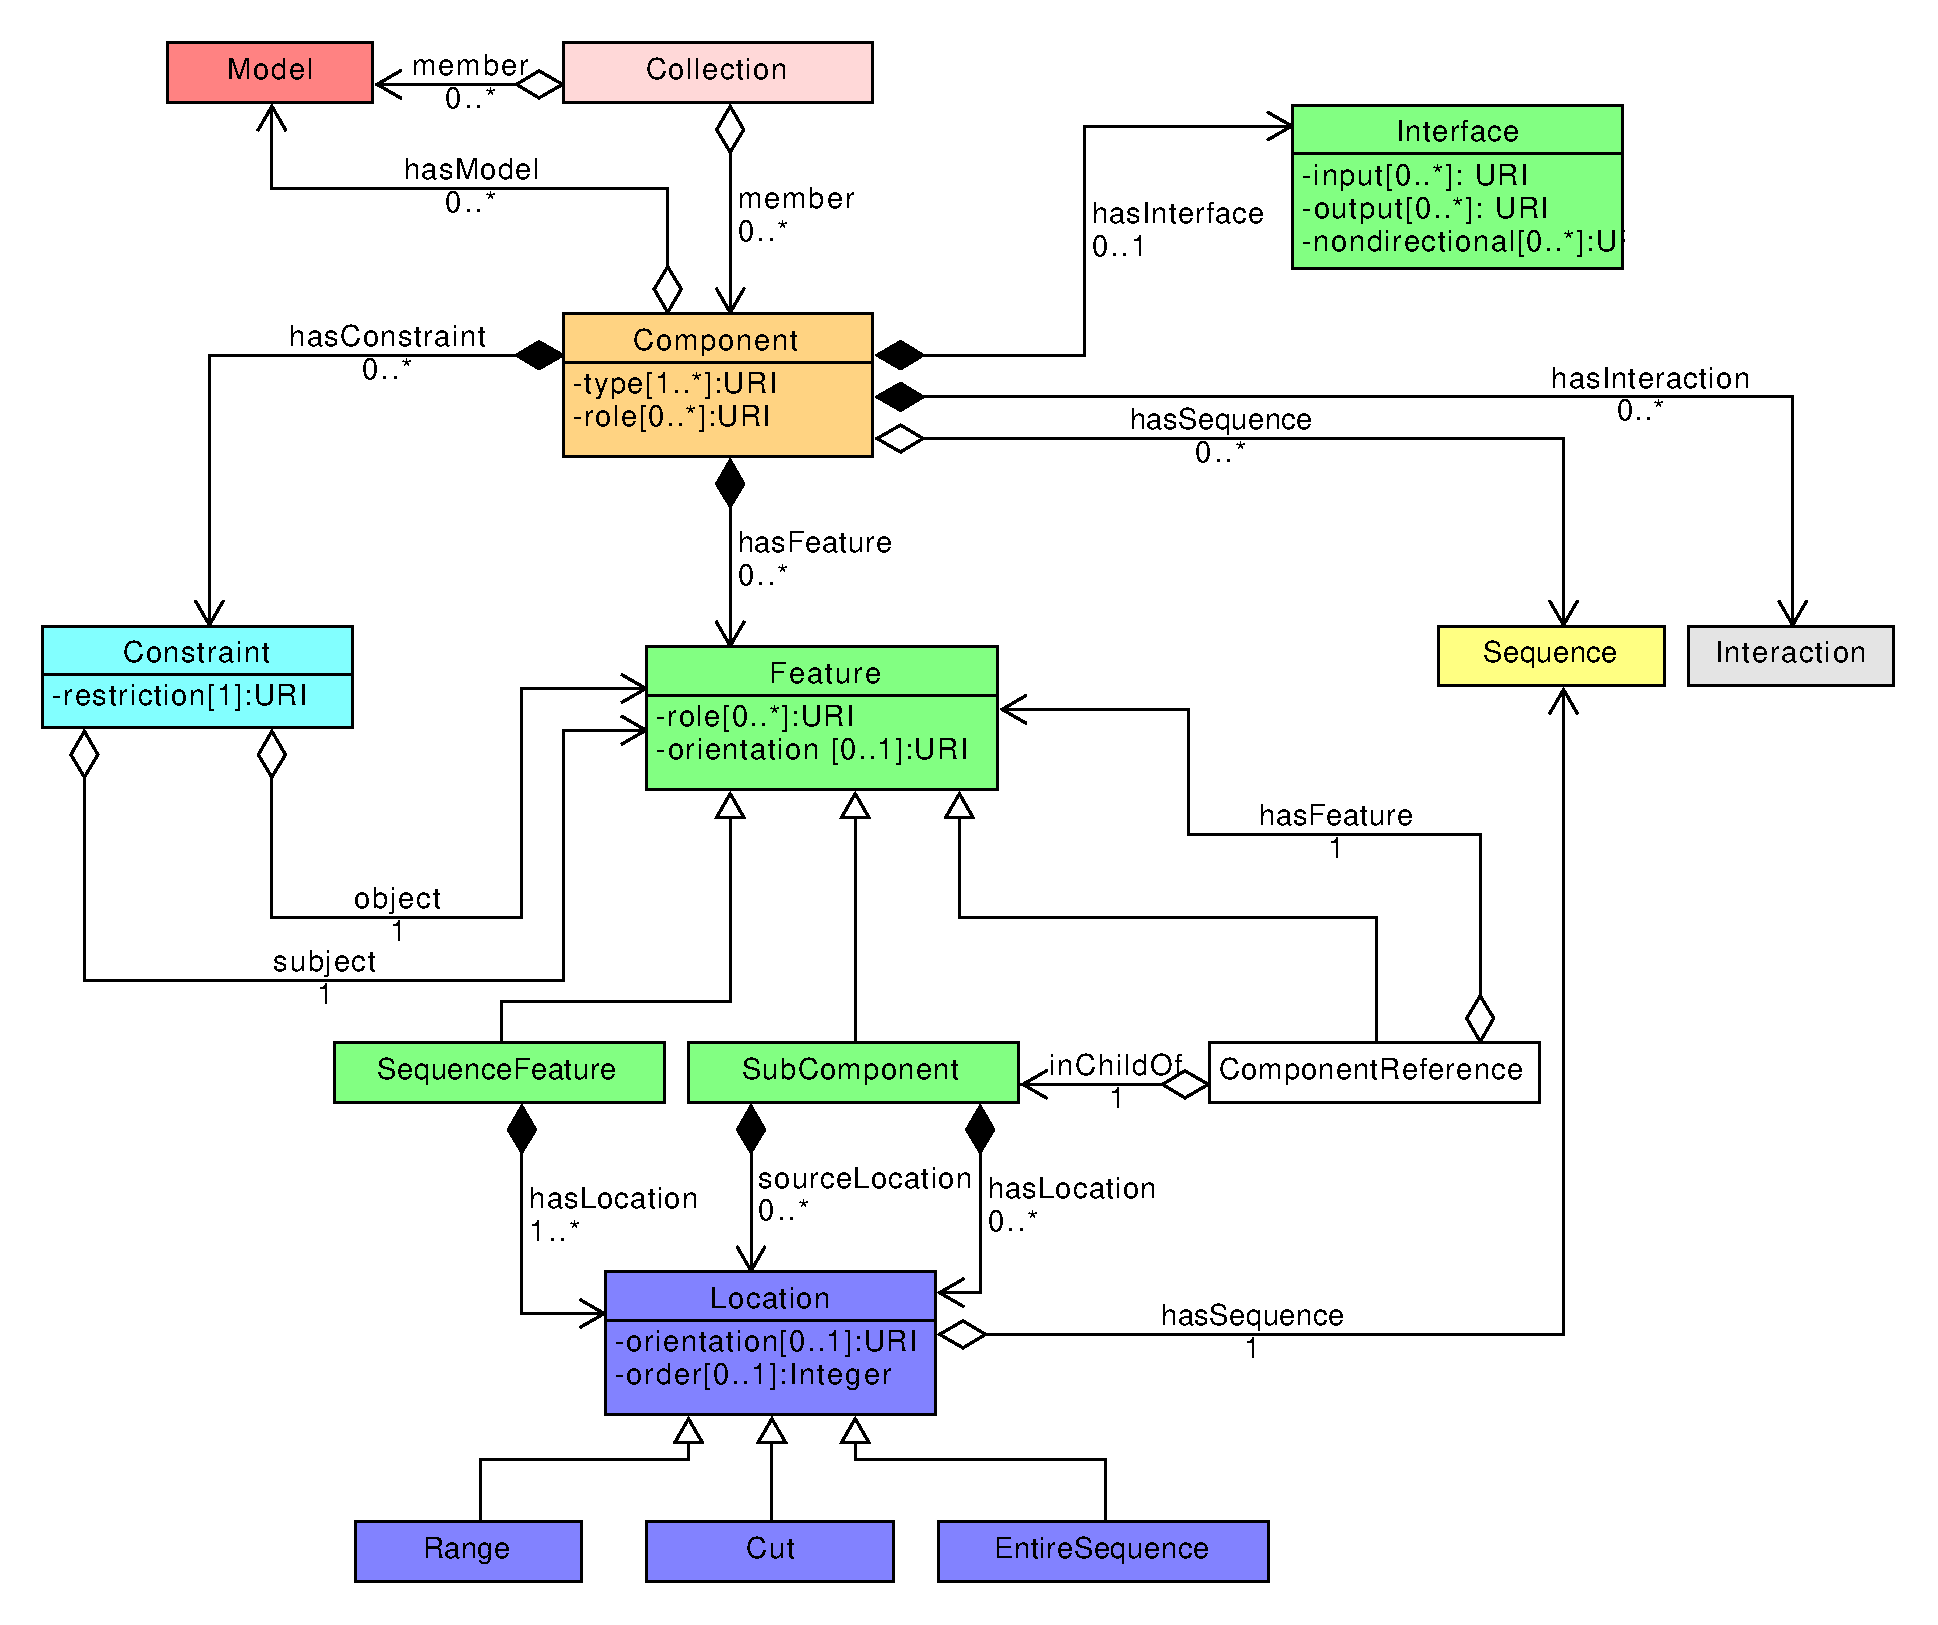
\includegraphics[width=0.8\linewidth]{uml/sbol_v2_to_v3_right_subfigure}  
		\caption{SBOL 3.x}
		\label{fig:sub-second}
	\end{subfigure}
	\caption{\label{SBOL2TO3}The mapping from the SBOL 2.3 data model to the SBOL 3.x  data model, indicating corresponding classes/properties by color.}
\end{figure*}
